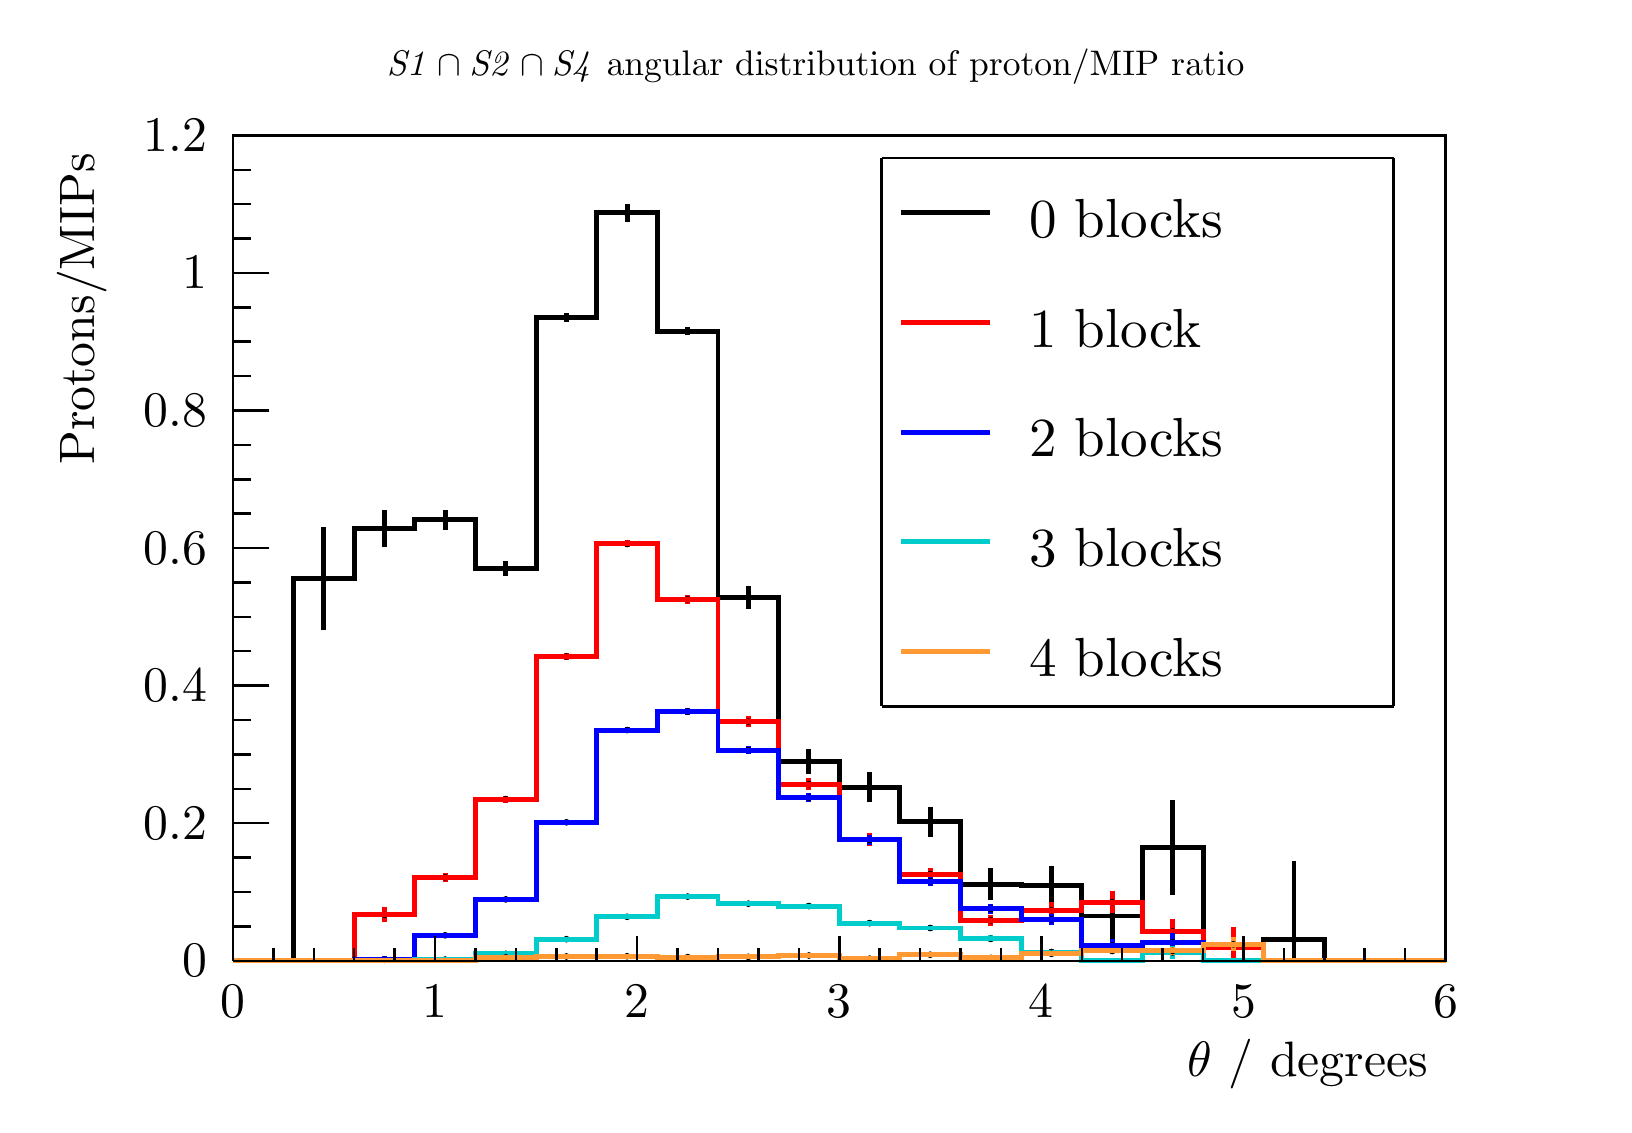
\begin{tikzpicture}
\pgfdeclareplotmark{cross} {
\pgfpathmoveto{\pgfpoint{-0.3\pgfplotmarksize}{\pgfplotmarksize}}
\pgfpathlineto{\pgfpoint{+0.3\pgfplotmarksize}{\pgfplotmarksize}}
\pgfpathlineto{\pgfpoint{+0.3\pgfplotmarksize}{0.3\pgfplotmarksize}}
\pgfpathlineto{\pgfpoint{+1\pgfplotmarksize}{0.3\pgfplotmarksize}}
\pgfpathlineto{\pgfpoint{+1\pgfplotmarksize}{-0.3\pgfplotmarksize}}
\pgfpathlineto{\pgfpoint{+0.3\pgfplotmarksize}{-0.3\pgfplotmarksize}}
\pgfpathlineto{\pgfpoint{+0.3\pgfplotmarksize}{-1.\pgfplotmarksize}}
\pgfpathlineto{\pgfpoint{-0.3\pgfplotmarksize}{-1.\pgfplotmarksize}}
\pgfpathlineto{\pgfpoint{-0.3\pgfplotmarksize}{-0.3\pgfplotmarksize}}
\pgfpathlineto{\pgfpoint{-1.\pgfplotmarksize}{-0.3\pgfplotmarksize}}
\pgfpathlineto{\pgfpoint{-1.\pgfplotmarksize}{0.3\pgfplotmarksize}}
\pgfpathlineto{\pgfpoint{-0.3\pgfplotmarksize}{0.3\pgfplotmarksize}}
\pgfpathclose
\pgfusepathqstroke
}
\pgfdeclareplotmark{cross*} {
\pgfpathmoveto{\pgfpoint{-0.3\pgfplotmarksize}{\pgfplotmarksize}}
\pgfpathlineto{\pgfpoint{+0.3\pgfplotmarksize}{\pgfplotmarksize}}
\pgfpathlineto{\pgfpoint{+0.3\pgfplotmarksize}{0.3\pgfplotmarksize}}
\pgfpathlineto{\pgfpoint{+1\pgfplotmarksize}{0.3\pgfplotmarksize}}
\pgfpathlineto{\pgfpoint{+1\pgfplotmarksize}{-0.3\pgfplotmarksize}}
\pgfpathlineto{\pgfpoint{+0.3\pgfplotmarksize}{-0.3\pgfplotmarksize}}
\pgfpathlineto{\pgfpoint{+0.3\pgfplotmarksize}{-1.\pgfplotmarksize}}
\pgfpathlineto{\pgfpoint{-0.3\pgfplotmarksize}{-1.\pgfplotmarksize}}
\pgfpathlineto{\pgfpoint{-0.3\pgfplotmarksize}{-0.3\pgfplotmarksize}}
\pgfpathlineto{\pgfpoint{-1.\pgfplotmarksize}{-0.3\pgfplotmarksize}}
\pgfpathlineto{\pgfpoint{-1.\pgfplotmarksize}{0.3\pgfplotmarksize}}
\pgfpathlineto{\pgfpoint{-0.3\pgfplotmarksize}{0.3\pgfplotmarksize}}
\pgfpathclose
\pgfusepathqfillstroke
}
\pgfdeclareplotmark{newstar} {
\pgfpathmoveto{\pgfqpoint{0pt}{\pgfplotmarksize}}
\pgfpathlineto{\pgfqpointpolar{44}{0.5\pgfplotmarksize}}
\pgfpathlineto{\pgfqpointpolar{18}{\pgfplotmarksize}}
\pgfpathlineto{\pgfqpointpolar{-20}{0.5\pgfplotmarksize}}
\pgfpathlineto{\pgfqpointpolar{-54}{\pgfplotmarksize}}
\pgfpathlineto{\pgfqpointpolar{-90}{0.5\pgfplotmarksize}}
\pgfpathlineto{\pgfqpointpolar{234}{\pgfplotmarksize}}
\pgfpathlineto{\pgfqpointpolar{198}{0.5\pgfplotmarksize}}
\pgfpathlineto{\pgfqpointpolar{162}{\pgfplotmarksize}}
\pgfpathlineto{\pgfqpointpolar{134}{0.5\pgfplotmarksize}}
\pgfpathclose
\pgfusepathqstroke
}
\pgfdeclareplotmark{newstar*} {
\pgfpathmoveto{\pgfqpoint{0pt}{\pgfplotmarksize}}
\pgfpathlineto{\pgfqpointpolar{44}{0.5\pgfplotmarksize}}
\pgfpathlineto{\pgfqpointpolar{18}{\pgfplotmarksize}}
\pgfpathlineto{\pgfqpointpolar{-20}{0.5\pgfplotmarksize}}
\pgfpathlineto{\pgfqpointpolar{-54}{\pgfplotmarksize}}
\pgfpathlineto{\pgfqpointpolar{-90}{0.5\pgfplotmarksize}}
\pgfpathlineto{\pgfqpointpolar{234}{\pgfplotmarksize}}
\pgfpathlineto{\pgfqpointpolar{198}{0.5\pgfplotmarksize}}
\pgfpathlineto{\pgfqpointpolar{162}{\pgfplotmarksize}}
\pgfpathlineto{\pgfqpointpolar{134}{0.5\pgfplotmarksize}}
\pgfpathclose
\pgfusepathqfillstroke
}
\definecolor{c}{rgb}{1,1,1};
\draw [color=c, fill=c] (0,0) rectangle (20,13.6127);
\draw [color=c, fill=c] (2.6,1.76965) rectangle (18,12.2514);
\definecolor{c}{rgb}{0,0,0};
\draw [c,line width=0.9] (2.6,1.76965) -- (2.6,12.2514) -- (18,12.2514) -- (18,1.76965) -- (2.6,1.76965);
\definecolor{c}{rgb}{1,1,1};
\draw [color=c, fill=c] (2.6,1.76965) rectangle (18,12.2514);
\definecolor{c}{rgb}{0,0,0};
\draw [c,line width=0.9] (2.6,1.76965) -- (2.6,12.2514) -- (18,12.2514) -- (18,1.76965) -- (2.6,1.76965);
\definecolor{c}{rgb}{0,0,0.6};
\draw [c,line width=0.9] (2.6,1.76965) -- (3.37,1.76965) -- (3.37,1.76965) -- (4.14,1.76965) -- (4.14,1.76965) -- (4.91,1.76965) -- (4.91,1.76965) -- (5.68,1.76965) -- (5.68,1.76965) -- (6.45,1.76965) -- (6.45,1.76965) -- (7.22,1.76965) --
 (7.22,1.76965) -- (7.99,1.76965) -- (7.99,1.76965) -- (8.76,1.76965) -- (8.76,1.76965) -- (9.53,1.76965) -- (9.53,1.76965) -- (10.3,1.76965) -- (10.3,1.76965) -- (11.07,1.76965) -- (11.07,1.76965) -- (11.84,1.76965) -- (11.84,1.76965) --
 (12.61,1.76965) -- (12.61,1.76965) -- (13.38,1.76965) -- (13.38,1.76965) -- (14.15,1.76965) -- (14.15,1.76965) -- (14.92,1.76965) -- (14.92,1.76965) -- (15.69,1.76965) -- (15.69,1.76965) -- (16.46,1.76965) -- (16.46,1.76965) -- (17.23,1.76965) --
 (17.23,1.76965) -- (18,1.76965);
\definecolor{c}{rgb}{0,0,0};
\draw [c,line width=0.9] (2.6,1.76965) -- (18,1.76965);
\draw [c,line width=0.9] (2.6,2.08411) -- (2.6,1.76965);
\draw [c,line width=0.9] (3.11333,1.92688) -- (3.11333,1.76965);
\draw [c,line width=0.9] (3.62667,1.92688) -- (3.62667,1.76965);
\draw [c,line width=0.9] (4.14,1.92688) -- (4.14,1.76965);
\draw [c,line width=0.9] (4.65333,1.92688) -- (4.65333,1.76965);
\draw [c,line width=0.9] (5.16667,2.08411) -- (5.16667,1.76965);
\draw [c,line width=0.9] (5.68,1.92688) -- (5.68,1.76965);
\draw [c,line width=0.9] (6.19333,1.92688) -- (6.19333,1.76965);
\draw [c,line width=0.9] (6.70667,1.92688) -- (6.70667,1.76965);
\draw [c,line width=0.9] (7.22,1.92688) -- (7.22,1.76965);
\draw [c,line width=0.9] (7.73333,2.08411) -- (7.73333,1.76965);
\draw [c,line width=0.9] (8.24667,1.92688) -- (8.24667,1.76965);
\draw [c,line width=0.9] (8.76,1.92688) -- (8.76,1.76965);
\draw [c,line width=0.9] (9.27333,1.92688) -- (9.27333,1.76965);
\draw [c,line width=0.9] (9.78667,1.92688) -- (9.78667,1.76965);
\draw [c,line width=0.9] (10.3,2.08411) -- (10.3,1.76965);
\draw [c,line width=0.9] (10.8133,1.92688) -- (10.8133,1.76965);
\draw [c,line width=0.9] (11.3267,1.92688) -- (11.3267,1.76965);
\draw [c,line width=0.9] (11.84,1.92688) -- (11.84,1.76965);
\draw [c,line width=0.9] (12.3533,1.92688) -- (12.3533,1.76965);
\draw [c,line width=0.9] (12.8667,2.08411) -- (12.8667,1.76965);
\draw [c,line width=0.9] (13.38,1.92688) -- (13.38,1.76965);
\draw [c,line width=0.9] (13.8933,1.92688) -- (13.8933,1.76965);
\draw [c,line width=0.9] (14.4067,1.92688) -- (14.4067,1.76965);
\draw [c,line width=0.9] (14.92,1.92688) -- (14.92,1.76965);
\draw [c,line width=0.9] (15.4333,2.08411) -- (15.4333,1.76965);
\draw [c,line width=0.9] (15.9467,1.92688) -- (15.9467,1.76965);
\draw [c,line width=0.9] (16.46,1.92688) -- (16.46,1.76965);
\draw [c,line width=0.9] (16.9733,1.92688) -- (16.9733,1.76965);
\draw [c,line width=0.9] (17.4867,1.92688) -- (17.4867,1.76965);
\draw [c,line width=0.9] (18,2.08411) -- (18,1.76965);
\draw [anchor=base] (2.6,1.04818) node[scale=1.79732, color=c, rotate=0]{0};
\draw [anchor=base] (5.16667,1.04818) node[scale=1.79732, color=c, rotate=0]{1};
\draw [anchor=base] (7.73333,1.04818) node[scale=1.79732, color=c, rotate=0]{2};
\draw [anchor=base] (10.3,1.04818) node[scale=1.79732, color=c, rotate=0]{3};
\draw [anchor=base] (12.8667,1.04818) node[scale=1.79732, color=c, rotate=0]{4};
\draw [anchor=base] (15.4333,1.04818) node[scale=1.79732, color=c, rotate=0]{5};
\draw [anchor=base] (18,1.04818) node[scale=1.79732, color=c, rotate=0]{6};
\draw [anchor= east] (18,0.462832) node[scale=1.79732, color=c, rotate=0]{$\theta$ / degrees};
\draw [c,line width=0.9] (2.6,1.76965) -- (2.6,12.2514);
\draw [c,line width=0.9] (3.062,1.76965) -- (2.6,1.76965);
\draw [c,line width=0.9] (2.831,2.20639) -- (2.6,2.20639);
\draw [c,line width=0.9] (2.831,2.64314) -- (2.6,2.64314);
\draw [c,line width=0.9] (2.831,3.07988) -- (2.6,3.07988);
\draw [c,line width=0.9] (3.062,3.51662) -- (2.6,3.51662);
\draw [c,line width=0.9] (2.831,3.95336) -- (2.6,3.95336);
\draw [c,line width=0.9] (2.831,4.3901) -- (2.6,4.3901);
\draw [c,line width=0.9] (2.831,4.82684) -- (2.6,4.82684);
\draw [c,line width=0.9] (3.062,5.26358) -- (2.6,5.26358);
\draw [c,line width=0.9] (2.831,5.70033) -- (2.6,5.70033);
\draw [c,line width=0.9] (2.831,6.13707) -- (2.6,6.13707);
\draw [c,line width=0.9] (2.831,6.57381) -- (2.6,6.57381);
\draw [c,line width=0.9] (3.062,7.01055) -- (2.6,7.01055);
\draw [c,line width=0.9] (2.831,7.44729) -- (2.6,7.44729);
\draw [c,line width=0.9] (2.831,7.88403) -- (2.6,7.88403);
\draw [c,line width=0.9] (2.831,8.32077) -- (2.6,8.32077);
\draw [c,line width=0.9] (3.062,8.75751) -- (2.6,8.75751);
\draw [c,line width=0.9] (2.831,9.19426) -- (2.6,9.19426);
\draw [c,line width=0.9] (2.831,9.631) -- (2.6,9.631);
\draw [c,line width=0.9] (2.831,10.0677) -- (2.6,10.0677);
\draw [c,line width=0.9] (3.062,10.5045) -- (2.6,10.5045);
\draw [c,line width=0.9] (2.831,10.9412) -- (2.6,10.9412);
\draw [c,line width=0.9] (2.831,11.378) -- (2.6,11.378);
\draw [c,line width=0.9] (2.831,11.8147) -- (2.6,11.8147);
\draw [c,line width=0.9] (3.062,12.2514) -- (2.6,12.2514);
\draw [c,line width=0.9] (3.062,12.2514) -- (2.6,12.2514);
\draw [anchor= east] (2.5,1.76965) node[scale=1.79732, color=c, rotate=0]{0};
\draw [anchor= east] (2.5,3.51662) node[scale=1.79732, color=c, rotate=0]{0.2};
\draw [anchor= east] (2.5,5.26358) node[scale=1.79732, color=c, rotate=0]{0.4};
\draw [anchor= east] (2.5,7.01055) node[scale=1.79732, color=c, rotate=0]{0.6};
\draw [anchor= east] (2.5,8.75751) node[scale=1.79732, color=c, rotate=0]{0.8};
\draw [anchor= east] (2.5,10.5045) node[scale=1.79732, color=c, rotate=0]{1};
\draw [anchor= east] (2.5,12.2514) node[scale=1.79732, color=c, rotate=0]{1.2};
\draw [anchor= east] (0.68,12.2514) node[scale=1.79732, color=c, rotate=90]{ Protons/MIPs};
\draw [c,line width=1.8] (3.755,5.96552) -- (3.755,6.61918);
\draw [c,line width=1.8] (3.755,6.61918) -- (3.755,7.27284);
\foreach \P in {(3.755,6.61918)}{\draw[mark options={color=c,fill=c},mark size=2.402402pt,mark=*,mark size=1pt] plot coordinates {\P};}
\draw [c,line width=1.8] (4.525,7.02017) -- (4.525,7.25485);
\draw [c,line width=1.8] (4.525,7.25485) -- (4.525,7.48953);
\foreach \P in {(4.525,7.25485)}{\draw[mark options={color=c,fill=c},mark size=2.402402pt,mark=*,mark size=1pt] plot coordinates {\P};}
\draw [c,line width=1.8] (5.295,7.24454) -- (5.295,7.36993);
\draw [c,line width=1.8] (5.295,7.36993) -- (5.295,7.49531);
\foreach \P in {(5.295,7.36993)}{\draw[mark options={color=c,fill=c},mark size=2.402402pt,mark=*,mark size=1pt] plot coordinates {\P};}
\draw [c,line width=1.8] (6.065,6.65801) -- (6.065,6.75329);
\draw [c,line width=1.8] (6.065,6.75329) -- (6.065,6.84857);
\foreach \P in {(6.065,6.75329)}{\draw[mark options={color=c,fill=c},mark size=2.402402pt,mark=*,mark size=1pt] plot coordinates {\P};}
\draw [c,line width=1.8] (6.835,9.88682) -- (6.835,9.94428);
\draw [c,line width=1.8] (6.835,9.94428) -- (6.835,10.0017);
\foreach \P in {(6.835,9.94428)}{\draw[mark options={color=c,fill=c},mark size=2.402402pt,mark=*,mark size=1pt] plot coordinates {\P};}
\draw [c,line width=1.8] (7.605,11.157) -- (7.605,11.267);
\draw [c,line width=1.8] (7.605,11.267) -- (7.605,11.3769);
\foreach \P in {(7.605,11.267)}{\draw[mark options={color=c,fill=c},mark size=2.402402pt,mark=*,mark size=1pt] plot coordinates {\P};}
\draw [c,line width=1.8] (8.375,9.71118) -- (8.375,9.76656);
\draw [c,line width=1.8] (8.375,9.76656) -- (8.375,9.82195);
\foreach \P in {(8.375,9.76656)}{\draw[mark options={color=c,fill=c},mark size=2.402402pt,mark=*,mark size=1pt] plot coordinates {\P};}
\draw [c,line width=1.8] (9.145,6.23982) -- (9.145,6.3858);
\draw [c,line width=1.8] (9.145,6.3858) -- (9.145,6.53178);
\foreach \P in {(9.145,6.3858)}{\draw[mark options={color=c,fill=c},mark size=2.402402pt,mark=*,mark size=1pt] plot coordinates {\P};}
\draw [c,line width=1.8] (9.915,4.14538) -- (9.915,4.30397);
\draw [c,line width=1.8] (9.915,4.30397) -- (9.915,4.46257);
\foreach \P in {(9.915,4.30397)}{\draw[mark options={color=c,fill=c},mark size=2.402402pt,mark=*,mark size=1pt] plot coordinates {\P};}
\draw [c,line width=1.8] (10.685,3.78343) -- (10.685,3.9732);
\draw [c,line width=1.8] (10.685,3.9732) -- (10.685,4.16297);
\foreach \P in {(10.685,3.9732)}{\draw[mark options={color=c,fill=c},mark size=2.402402pt,mark=*,mark size=1pt] plot coordinates {\P};}
\draw [c,line width=1.8] (11.455,3.3397) -- (11.455,3.53224);
\draw [c,line width=1.8] (11.455,3.53224) -- (11.455,3.72478);
\foreach \P in {(11.455,3.53224)}{\draw[mark options={color=c,fill=c},mark size=2.402402pt,mark=*,mark size=1pt] plot coordinates {\P};}
\draw [c,line width=1.8] (12.225,2.53805) -- (12.225,2.74072);
\draw [c,line width=1.8] (12.225,2.74072) -- (12.225,2.94338);
\foreach \P in {(12.225,2.74072)}{\draw[mark options={color=c,fill=c},mark size=2.402402pt,mark=*,mark size=1pt] plot coordinates {\P};}
\draw [c,line width=1.8] (12.995,2.48276) -- (12.995,2.72628);
\draw [c,line width=1.8] (12.995,2.72628) -- (12.995,2.9698);
\foreach \P in {(12.995,2.72628)}{\draw[mark options={color=c,fill=c},mark size=2.402402pt,mark=*,mark size=1pt] plot coordinates {\P};}
\draw [c,line width=1.8] (13.765,2.01881) -- (13.765,2.3379);
\draw [c,line width=1.8] (13.765,2.3379) -- (13.765,2.65699);
\foreach \P in {(13.765,2.3379)}{\draw[mark options={color=c,fill=c},mark size=2.402402pt,mark=*,mark size=1pt] plot coordinates {\P};}
\draw [c,line width=1.8] (14.535,2.60709) -- (14.535,3.20937);
\draw [c,line width=1.8] (14.535,3.20937) -- (14.535,3.81165);
\foreach \P in {(14.535,3.20937)}{\draw[mark options={color=c,fill=c},mark size=2.402402pt,mark=*,mark size=1pt] plot coordinates {\P};}
\draw [c,line width=1.8] (16.075,1.76965) -- (16.075,2.03461);
\draw [c,line width=1.8] (16.075,2.03461) -- (16.075,3.04084);
\foreach \P in {(16.075,2.03461)}{\draw[mark options={color=c,fill=c},mark size=2.402402pt,mark=*,mark size=1pt] plot coordinates {\P};}
\draw [c,line width=1.8] (2.6,1.76965) -- (3.37,1.76965) -- (3.37,6.61918) -- (4.14,6.61918) -- (4.14,7.25485) -- (4.91,7.25485) -- (4.91,7.36993) -- (5.68,7.36993) -- (5.68,6.75329) -- (6.45,6.75329) -- (6.45,9.94428) -- (7.22,9.94428) --
 (7.22,11.267) -- (7.99,11.267) -- (7.99,9.76656) -- (8.76,9.76656) -- (8.76,6.3858) -- (9.53,6.3858) -- (9.53,4.30397) -- (10.3,4.30397) -- (10.3,3.9732) -- (11.07,3.9732) -- (11.07,3.53224) -- (11.84,3.53224) -- (11.84,2.74072) -- (12.61,2.74072)
 -- (12.61,2.72628) -- (13.38,2.72628) -- (13.38,2.3379) -- (14.15,2.3379) -- (14.15,3.20937) -- (14.92,3.20937) -- (14.92,1.76965) -- (15.69,1.76965) -- (15.69,2.03461) -- (16.46,2.03461) -- (16.46,1.76965) -- (17.23,1.76965) -- (17.23,1.76965) --
 (18,1.76965);
\definecolor{c}{rgb}{1,0,0};
\draw [c,line width=1.8] (4.525,2.25718) -- (4.525,2.35159);
\draw [c,line width=1.8] (4.525,2.35159) -- (4.525,2.446);
\definecolor{c}{rgb}{0,0,0};
\foreach \P in {(4.525,2.35159)}{\draw[mark options={color=c,fill=c},mark size=2.402402pt,mark=*,mark size=1pt] plot coordinates {\P};}
\definecolor{c}{rgb}{1,0,0};
\draw [c,line width=1.8] (5.295,2.77091) -- (5.295,2.82905);
\draw [c,line width=1.8] (5.295,2.82905) -- (5.295,2.88719);
\definecolor{c}{rgb}{0,0,0};
\foreach \P in {(5.295,2.82905)}{\draw[mark options={color=c,fill=c},mark size=2.402402pt,mark=*,mark size=1pt] plot coordinates {\P};}
\definecolor{c}{rgb}{1,0,0};
\draw [c,line width=1.8] (6.065,3.77647) -- (6.065,3.82233);
\draw [c,line width=1.8] (6.065,3.82233) -- (6.065,3.86819);
\definecolor{c}{rgb}{0,0,0};
\foreach \P in {(6.065,3.82233)}{\draw[mark options={color=c,fill=c},mark size=2.402402pt,mark=*,mark size=1pt] plot coordinates {\P};}
\definecolor{c}{rgb}{1,0,0};
\draw [c,line width=1.8] (6.835,5.59037) -- (6.835,5.63438);
\draw [c,line width=1.8] (6.835,5.63438) -- (6.835,5.67838);
\definecolor{c}{rgb}{0,0,0};
\foreach \P in {(6.835,5.63438)}{\draw[mark options={color=c,fill=c},mark size=2.402402pt,mark=*,mark size=1pt] plot coordinates {\P};}
\definecolor{c}{rgb}{1,0,0};
\draw [c,line width=1.8] (7.605,7.01849) -- (7.605,7.06322);
\draw [c,line width=1.8] (7.605,7.06322) -- (7.605,7.10796);
\definecolor{c}{rgb}{0,0,0};
\foreach \P in {(7.605,7.06322)}{\draw[mark options={color=c,fill=c},mark size=2.402402pt,mark=*,mark size=1pt] plot coordinates {\P};}
\definecolor{c}{rgb}{1,0,0};
\draw [c,line width=1.8] (8.375,6.30504) -- (8.375,6.36061);
\draw [c,line width=1.8] (8.375,6.36061) -- (8.375,6.41618);
\definecolor{c}{rgb}{0,0,0};
\foreach \P in {(8.375,6.36061)}{\draw[mark options={color=c,fill=c},mark size=2.402402pt,mark=*,mark size=1pt] plot coordinates {\P};}
\definecolor{c}{rgb}{1,0,0};
\draw [c,line width=1.8] (9.145,4.73795) -- (9.145,4.80704);
\draw [c,line width=1.8] (9.145,4.80704) -- (9.145,4.87612);
\definecolor{c}{rgb}{0,0,0};
\foreach \P in {(9.145,4.80704)}{\draw[mark options={color=c,fill=c},mark size=2.402402pt,mark=*,mark size=1pt] plot coordinates {\P};}
\definecolor{c}{rgb}{1,0,0};
\draw [c,line width=1.8] (9.915,3.93827) -- (9.915,4.01338);
\draw [c,line width=1.8] (9.915,4.01338) -- (9.915,4.08848);
\definecolor{c}{rgb}{0,0,0};
\foreach \P in {(9.915,4.01338)}{\draw[mark options={color=c,fill=c},mark size=2.402402pt,mark=*,mark size=1pt] plot coordinates {\P};}
\definecolor{c}{rgb}{1,0,0};
\draw [c,line width=1.8] (10.685,3.22568) -- (10.685,3.30686);
\draw [c,line width=1.8] (10.685,3.30686) -- (10.685,3.38804);
\definecolor{c}{rgb}{0,0,0};
\foreach \P in {(10.685,3.30686)}{\draw[mark options={color=c,fill=c},mark size=2.402402pt,mark=*,mark size=1pt] plot coordinates {\P};}
\definecolor{c}{rgb}{1,0,0};
\draw [c,line width=1.8] (11.455,2.78746) -- (11.455,2.87067);
\draw [c,line width=1.8] (11.455,2.87067) -- (11.455,2.95388);
\definecolor{c}{rgb}{0,0,0};
\foreach \P in {(11.455,2.87067)}{\draw[mark options={color=c,fill=c},mark size=2.402402pt,mark=*,mark size=1pt] plot coordinates {\P};}
\definecolor{c}{rgb}{1,0,0};
\draw [c,line width=1.8] (12.225,2.21253) -- (12.225,2.28363);
\draw [c,line width=1.8] (12.225,2.28363) -- (12.225,2.35473);
\definecolor{c}{rgb}{0,0,0};
\foreach \P in {(12.225,2.28363)}{\draw[mark options={color=c,fill=c},mark size=2.402402pt,mark=*,mark size=1pt] plot coordinates {\P};}
\definecolor{c}{rgb}{1,0,0};
\draw [c,line width=1.8] (12.995,2.30897) -- (12.995,2.41012);
\draw [c,line width=1.8] (12.995,2.41012) -- (12.995,2.51127);
\definecolor{c}{rgb}{0,0,0};
\foreach \P in {(12.995,2.41012)}{\draw[mark options={color=c,fill=c},mark size=2.402402pt,mark=*,mark size=1pt] plot coordinates {\P};}
\definecolor{c}{rgb}{1,0,0};
\draw [c,line width=1.8] (13.765,2.37186) -- (13.765,2.51465);
\draw [c,line width=1.8] (13.765,2.51465) -- (13.765,2.65744);
\definecolor{c}{rgb}{0,0,0};
\foreach \P in {(13.765,2.51465)}{\draw[mark options={color=c,fill=c},mark size=2.402402pt,mark=*,mark size=1pt] plot coordinates {\P};}
\definecolor{c}{rgb}{1,0,0};
\draw [c,line width=1.8] (14.535,1.98578) -- (14.535,2.14154);
\draw [c,line width=1.8] (14.535,2.14154) -- (14.535,2.29731);
\definecolor{c}{rgb}{0,0,0};
\foreach \P in {(14.535,2.14154)}{\draw[mark options={color=c,fill=c},mark size=2.402402pt,mark=*,mark size=1pt] plot coordinates {\P};}
\definecolor{c}{rgb}{1,0,0};
\draw [c,line width=1.8] (15.305,1.76965) -- (15.305,1.94371);
\draw [c,line width=1.8] (15.305,1.94371) -- (15.305,2.19744);
\definecolor{c}{rgb}{0,0,0};
\foreach \P in {(15.305,1.94371)}{\draw[mark options={color=c,fill=c},mark size=2.402402pt,mark=*,mark size=1pt] plot coordinates {\P};}
\definecolor{c}{rgb}{1,0,0};
\draw [c,line width=1.8] (2.6,1.76965) -- (3.37,1.76965) -- (3.37,1.76965) -- (4.14,1.76965) -- (4.14,2.35159) -- (4.91,2.35159) -- (4.91,2.82905) -- (5.68,2.82905) -- (5.68,3.82233) -- (6.45,3.82233) -- (6.45,5.63438) -- (7.22,5.63438) --
 (7.22,7.06322) -- (7.99,7.06322) -- (7.99,6.36061) -- (8.76,6.36061) -- (8.76,4.80704) -- (9.53,4.80704) -- (9.53,4.01338) -- (10.3,4.01338) -- (10.3,3.30686) -- (11.07,3.30686) -- (11.07,2.87067) -- (11.84,2.87067) -- (11.84,2.28363) --
 (12.61,2.28363) -- (12.61,2.41012) -- (13.38,2.41012) -- (13.38,2.51465) -- (14.15,2.51465) -- (14.15,2.14154) -- (14.92,2.14154) -- (14.92,1.94371) -- (15.69,1.94371) -- (15.69,1.76965) -- (16.46,1.76965) -- (16.46,1.76965) -- (17.23,1.76965) --
 (17.23,1.76965) -- (18,1.76965);
\definecolor{c}{rgb}{0,0,1};
\draw [c,line width=1.8] (4.525,1.76965) -- (4.525,1.7823);
\draw [c,line width=1.8] (4.525,1.7823) -- (4.525,1.83564);
\definecolor{c}{rgb}{0,0,0};
\foreach \P in {(4.525,1.7823)}{\draw[mark options={color=c,fill=c},mark size=2.402402pt,mark=*,mark size=1pt] plot coordinates {\P};}
\definecolor{c}{rgb}{0,0,1};
\draw [c,line width=1.8] (5.295,2.06026) -- (5.295,2.09298);
\draw [c,line width=1.8] (5.295,2.09298) -- (5.295,2.12571);
\definecolor{c}{rgb}{0,0,0};
\foreach \P in {(5.295,2.09298)}{\draw[mark options={color=c,fill=c},mark size=2.402402pt,mark=*,mark size=1pt] plot coordinates {\P};}
\definecolor{c}{rgb}{0,0,1};
\draw [c,line width=1.8] (6.065,2.5215) -- (6.065,2.54923);
\draw [c,line width=1.8] (6.065,2.54923) -- (6.065,2.57695);
\definecolor{c}{rgb}{0,0,0};
\foreach \P in {(6.065,2.54923)}{\draw[mark options={color=c,fill=c},mark size=2.402402pt,mark=*,mark size=1pt] plot coordinates {\P};}
\definecolor{c}{rgb}{0,0,1};
\draw [c,line width=1.8] (6.835,3.49681) -- (6.835,3.52792);
\draw [c,line width=1.8] (6.835,3.52792) -- (6.835,3.55903);
\definecolor{c}{rgb}{0,0,0};
\foreach \P in {(6.835,3.52792)}{\draw[mark options={color=c,fill=c},mark size=2.402402pt,mark=*,mark size=1pt] plot coordinates {\P};}
\definecolor{c}{rgb}{0,0,1};
\draw [c,line width=1.8] (7.605,4.66274) -- (7.605,4.69928);
\draw [c,line width=1.8] (7.605,4.69928) -- (7.605,4.73582);
\definecolor{c}{rgb}{0,0,0};
\foreach \P in {(7.605,4.69928)}{\draw[mark options={color=c,fill=c},mark size=2.402402pt,mark=*,mark size=1pt] plot coordinates {\P};}
\definecolor{c}{rgb}{0,0,1};
\draw [c,line width=1.8] (8.375,4.89186) -- (8.375,4.93533);
\draw [c,line width=1.8] (8.375,4.93533) -- (8.375,4.9788);
\definecolor{c}{rgb}{0,0,0};
\foreach \P in {(8.375,4.93533)}{\draw[mark options={color=c,fill=c},mark size=2.402402pt,mark=*,mark size=1pt] plot coordinates {\P};}
\definecolor{c}{rgb}{0,0,1};
\draw [c,line width=1.8] (9.145,4.39433) -- (9.145,4.44478);
\draw [c,line width=1.8] (9.145,4.44478) -- (9.145,4.49524);
\definecolor{c}{rgb}{0,0,0};
\foreach \P in {(9.145,4.44478)}{\draw[mark options={color=c,fill=c},mark size=2.402402pt,mark=*,mark size=1pt] plot coordinates {\P};}
\definecolor{c}{rgb}{0,0,1};
\draw [c,line width=1.8] (9.915,3.78582) -- (9.915,3.84078);
\draw [c,line width=1.8] (9.915,3.84078) -- (9.915,3.89575);
\definecolor{c}{rgb}{0,0,0};
\foreach \P in {(9.915,3.84078)}{\draw[mark options={color=c,fill=c},mark size=2.402402pt,mark=*,mark size=1pt] plot coordinates {\P};}
\definecolor{c}{rgb}{0,0,1};
\draw [c,line width=1.8] (10.685,3.24461) -- (10.685,3.3036);
\draw [c,line width=1.8] (10.685,3.3036) -- (10.685,3.36259);
\definecolor{c}{rgb}{0,0,0};
\foreach \P in {(10.685,3.3036)}{\draw[mark options={color=c,fill=c},mark size=2.402402pt,mark=*,mark size=1pt] plot coordinates {\P};}
\definecolor{c}{rgb}{0,0,1};
\draw [c,line width=1.8] (11.455,2.72135) -- (11.455,2.77999);
\draw [c,line width=1.8] (11.455,2.77999) -- (11.455,2.83863);
\definecolor{c}{rgb}{0,0,0};
\foreach \P in {(11.455,2.77999)}{\draw[mark options={color=c,fill=c},mark size=2.402402pt,mark=*,mark size=1pt] plot coordinates {\P};}
\definecolor{c}{rgb}{0,0,1};
\draw [c,line width=1.8] (12.225,2.36619) -- (12.225,2.42732);
\draw [c,line width=1.8] (12.225,2.42732) -- (12.225,2.48844);
\definecolor{c}{rgb}{0,0,0};
\foreach \P in {(12.225,2.42732)}{\draw[mark options={color=c,fill=c},mark size=2.402402pt,mark=*,mark size=1pt] plot coordinates {\P};}
\definecolor{c}{rgb}{0,0,1};
\draw [c,line width=1.8] (12.995,2.22581) -- (12.995,2.29456);
\draw [c,line width=1.8] (12.995,2.29456) -- (12.995,2.36332);
\definecolor{c}{rgb}{0,0,0};
\foreach \P in {(12.995,2.29456)}{\draw[mark options={color=c,fill=c},mark size=2.402402pt,mark=*,mark size=1pt] plot coordinates {\P};}
\definecolor{c}{rgb}{0,0,1};
\draw [c,line width=1.8] (13.765,1.88797) -- (13.765,1.96423);
\draw [c,line width=1.8] (13.765,1.96423) -- (13.765,2.04048);
\definecolor{c}{rgb}{0,0,0};
\foreach \P in {(13.765,1.96423)}{\draw[mark options={color=c,fill=c},mark size=2.402402pt,mark=*,mark size=1pt] plot coordinates {\P};}
\definecolor{c}{rgb}{0,0,1};
\draw [c,line width=1.8] (14.535,1.88836) -- (14.535,2.00549);
\draw [c,line width=1.8] (14.535,2.00549) -- (14.535,2.12261);
\definecolor{c}{rgb}{0,0,0};
\foreach \P in {(14.535,2.00549)}{\draw[mark options={color=c,fill=c},mark size=2.402402pt,mark=*,mark size=1pt] plot coordinates {\P};}
\definecolor{c}{rgb}{0,0,1};
\draw [c,line width=1.8] (2.6,1.76965) -- (3.37,1.76965) -- (3.37,1.76965) -- (4.14,1.76965) -- (4.14,1.7823) -- (4.91,1.7823) -- (4.91,2.09298) -- (5.68,2.09298) -- (5.68,2.54923) -- (6.45,2.54923) -- (6.45,3.52792) -- (7.22,3.52792) --
 (7.22,4.69928) -- (7.99,4.69928) -- (7.99,4.93533) -- (8.76,4.93533) -- (8.76,4.44478) -- (9.53,4.44478) -- (9.53,3.84078) -- (10.3,3.84078) -- (10.3,3.3036) -- (11.07,3.3036) -- (11.07,2.77999) -- (11.84,2.77999) -- (11.84,2.42732) --
 (12.61,2.42732) -- (12.61,2.29456) -- (13.38,2.29456) -- (13.38,1.96423) -- (14.15,1.96423) -- (14.15,2.00549) -- (14.92,2.00549) -- (14.92,1.76965) -- (15.69,1.76965) -- (15.69,1.76965) -- (16.46,1.76965) -- (16.46,1.76965) -- (17.23,1.76965) --
 (17.23,1.76965) -- (18,1.76965);
\definecolor{c}{rgb}{0,0.8,0.8};
\draw [c,line width=1.8] (5.295,1.76965) -- (5.295,1.78457);
\draw [c,line width=1.8] (5.295,1.78457) -- (5.295,1.80271);
\definecolor{c}{rgb}{0,0,0};
\foreach \P in {(5.295,1.78457)}{\draw[mark options={color=c,fill=c},mark size=2.402402pt,mark=*,mark size=1pt] plot coordinates {\P};}
\definecolor{c}{rgb}{0,0.8,0.8};
\draw [c,line width=1.8] (6.065,1.8446) -- (6.065,1.8573);
\draw [c,line width=1.8] (6.065,1.8573) -- (6.065,1.87);
\definecolor{c}{rgb}{0,0,0};
\foreach \P in {(6.065,1.8573)}{\draw[mark options={color=c,fill=c},mark size=2.402402pt,mark=*,mark size=1pt] plot coordinates {\P};}
\definecolor{c}{rgb}{0,0.8,0.8};
\draw [c,line width=1.8] (6.835,2.02672) -- (6.835,2.04365);
\draw [c,line width=1.8] (6.835,2.04365) -- (6.835,2.06058);
\definecolor{c}{rgb}{0,0,0};
\foreach \P in {(6.835,2.04365)}{\draw[mark options={color=c,fill=c},mark size=2.402402pt,mark=*,mark size=1pt] plot coordinates {\P};}
\definecolor{c}{rgb}{0,0.8,0.8};
\draw [c,line width=1.8] (7.605,2.30633) -- (7.605,2.32789);
\draw [c,line width=1.8] (7.605,2.32789) -- (7.605,2.34945);
\definecolor{c}{rgb}{0,0,0};
\foreach \P in {(7.605,2.32789)}{\draw[mark options={color=c,fill=c},mark size=2.402402pt,mark=*,mark size=1pt] plot coordinates {\P};}
\definecolor{c}{rgb}{0,0.8,0.8};
\draw [c,line width=1.8] (8.375,2.55536) -- (8.375,2.58455);
\draw [c,line width=1.8] (8.375,2.58455) -- (8.375,2.61374);
\definecolor{c}{rgb}{0,0,0};
\foreach \P in {(8.375,2.58455)}{\draw[mark options={color=c,fill=c},mark size=2.402402pt,mark=*,mark size=1pt] plot coordinates {\P};}
\definecolor{c}{rgb}{0,0.8,0.8};
\draw [c,line width=1.8] (9.145,2.46079) -- (9.145,2.49448);
\draw [c,line width=1.8] (9.145,2.49448) -- (9.145,2.52816);
\definecolor{c}{rgb}{0,0,0};
\foreach \P in {(9.145,2.49448)}{\draw[mark options={color=c,fill=c},mark size=2.402402pt,mark=*,mark size=1pt] plot coordinates {\P};}
\definecolor{c}{rgb}{0,0.8,0.8};
\draw [c,line width=1.8] (9.915,2.42409) -- (9.915,2.46387);
\draw [c,line width=1.8] (9.915,2.46387) -- (9.915,2.50366);
\definecolor{c}{rgb}{0,0,0};
\foreach \P in {(9.915,2.46387)}{\draw[mark options={color=c,fill=c},mark size=2.402402pt,mark=*,mark size=1pt] plot coordinates {\P};}
\definecolor{c}{rgb}{0,0.8,0.8};
\draw [c,line width=1.8] (10.685,2.20946) -- (10.685,2.2468);
\draw [c,line width=1.8] (10.685,2.2468) -- (10.685,2.28414);
\definecolor{c}{rgb}{0,0,0};
\foreach \P in {(10.685,2.2468)}{\draw[mark options={color=c,fill=c},mark size=2.402402pt,mark=*,mark size=1pt] plot coordinates {\P};}
\definecolor{c}{rgb}{0,0.8,0.8};
\draw [c,line width=1.8] (11.455,2.14459) -- (11.455,2.18563);
\draw [c,line width=1.8] (11.455,2.18563) -- (11.455,2.22667);
\definecolor{c}{rgb}{0,0,0};
\foreach \P in {(11.455,2.18563)}{\draw[mark options={color=c,fill=c},mark size=2.402402pt,mark=*,mark size=1pt] plot coordinates {\P};}
\definecolor{c}{rgb}{0,0.8,0.8};
\draw [c,line width=1.8] (12.225,2.00237) -- (12.225,2.0483);
\draw [c,line width=1.8] (12.225,2.0483) -- (12.225,2.09422);
\definecolor{c}{rgb}{0,0,0};
\foreach \P in {(12.225,2.0483)}{\draw[mark options={color=c,fill=c},mark size=2.402402pt,mark=*,mark size=1pt] plot coordinates {\P};}
\definecolor{c}{rgb}{0,0.8,0.8};
\draw [c,line width=1.8] (12.995,1.8366) -- (12.995,1.8805);
\draw [c,line width=1.8] (12.995,1.8805) -- (12.995,1.92441);
\definecolor{c}{rgb}{0,0,0};
\foreach \P in {(12.995,1.8805)}{\draw[mark options={color=c,fill=c},mark size=2.402402pt,mark=*,mark size=1pt] plot coordinates {\P};}
\definecolor{c}{rgb}{0,0.8,0.8};
\draw [c,line width=1.8] (14.535,1.78926) -- (14.535,1.8749);
\draw [c,line width=1.8] (14.535,1.8749) -- (14.535,1.96054);
\definecolor{c}{rgb}{0,0,0};
\foreach \P in {(14.535,1.8749)}{\draw[mark options={color=c,fill=c},mark size=2.402402pt,mark=*,mark size=1pt] plot coordinates {\P};}
\definecolor{c}{rgb}{0,0.8,0.8};
\draw [c,line width=1.8] (2.6,1.76965) -- (3.37,1.76965) -- (3.37,1.76965) -- (4.14,1.76965) -- (4.14,1.76965) -- (4.91,1.76965) -- (4.91,1.78457) -- (5.68,1.78457) -- (5.68,1.8573) -- (6.45,1.8573) -- (6.45,2.04365) -- (7.22,2.04365) --
 (7.22,2.32789) -- (7.99,2.32789) -- (7.99,2.58455) -- (8.76,2.58455) -- (8.76,2.49448) -- (9.53,2.49448) -- (9.53,2.46387) -- (10.3,2.46387) -- (10.3,2.2468) -- (11.07,2.2468) -- (11.07,2.18563) -- (11.84,2.18563) -- (11.84,2.0483) -- (12.61,2.0483)
 -- (12.61,1.8805) -- (13.38,1.8805) -- (13.38,1.76965) -- (14.15,1.76965) -- (14.15,1.8749) -- (14.92,1.8749) -- (14.92,1.76965) -- (15.69,1.76965) -- (15.69,1.76965) -- (16.46,1.76965) -- (16.46,1.76965) -- (17.23,1.76965) -- (17.23,1.76965) --
 (18,1.76965);
\definecolor{c}{rgb}{1,0.6,0.2};
\draw [c,line width=1.8] (6.065,1.8082) -- (6.065,1.81294);
\draw [c,line width=1.8] (6.065,1.81294) -- (6.065,1.81769);
\definecolor{c}{rgb}{0,0,0};
\foreach \P in {(6.065,1.81294)}{\draw[mark options={color=c,fill=c},mark size=2.402402pt,mark=*,mark size=1pt] plot coordinates {\P};}
\definecolor{c}{rgb}{1,0.6,0.2};
\draw [c,line width=1.8] (6.835,1.81861) -- (6.835,1.82418);
\draw [c,line width=1.8] (6.835,1.82418) -- (6.835,1.82974);
\definecolor{c}{rgb}{0,0,0};
\foreach \P in {(6.835,1.82418)}{\draw[mark options={color=c,fill=c},mark size=2.402402pt,mark=*,mark size=1pt] plot coordinates {\P};}
\definecolor{c}{rgb}{1,0.6,0.2};
\draw [c,line width=1.8] (7.605,1.822) -- (7.605,1.82706);
\draw [c,line width=1.8] (7.605,1.82706) -- (7.605,1.83212);
\definecolor{c}{rgb}{0,0,0};
\foreach \P in {(7.605,1.82706)}{\draw[mark options={color=c,fill=c},mark size=2.402402pt,mark=*,mark size=1pt] plot coordinates {\P};}
\definecolor{c}{rgb}{1,0.6,0.2};
\draw [c,line width=1.8] (8.375,1.81073) -- (8.375,1.8155);
\draw [c,line width=1.8] (8.375,1.8155) -- (8.375,1.82027);
\definecolor{c}{rgb}{0,0,0};
\foreach \P in {(8.375,1.8155)}{\draw[mark options={color=c,fill=c},mark size=2.402402pt,mark=*,mark size=1pt] plot coordinates {\P};}
\definecolor{c}{rgb}{1,0.6,0.2};
\draw [c,line width=1.8] (9.145,1.81131) -- (9.145,1.81903);
\draw [c,line width=1.8] (9.145,1.81903) -- (9.145,1.82675);
\definecolor{c}{rgb}{0,0,0};
\foreach \P in {(9.145,1.81903)}{\draw[mark options={color=c,fill=c},mark size=2.402402pt,mark=*,mark size=1pt] plot coordinates {\P};}
\definecolor{c}{rgb}{1,0.6,0.2};
\draw [c,line width=1.8] (9.915,1.82508) -- (9.915,1.83644);
\draw [c,line width=1.8] (9.915,1.83644) -- (9.915,1.8478);
\definecolor{c}{rgb}{0,0,0};
\foreach \P in {(9.915,1.83644)}{\draw[mark options={color=c,fill=c},mark size=2.402402pt,mark=*,mark size=1pt] plot coordinates {\P};}
\definecolor{c}{rgb}{1,0.6,0.2};
\draw [c,line width=1.8] (10.685,1.79053) -- (10.685,1.79625);
\draw [c,line width=1.8] (10.685,1.79625) -- (10.685,1.80197);
\definecolor{c}{rgb}{0,0,0};
\foreach \P in {(10.685,1.79625)}{\draw[mark options={color=c,fill=c},mark size=2.402402pt,mark=*,mark size=1pt] plot coordinates {\P};}
\definecolor{c}{rgb}{1,0.6,0.2};
\draw [c,line width=1.8] (11.455,1.83001) -- (11.455,1.84612);
\draw [c,line width=1.8] (11.455,1.84612) -- (11.455,1.86223);
\definecolor{c}{rgb}{0,0,0};
\foreach \P in {(11.455,1.84612)}{\draw[mark options={color=c,fill=c},mark size=2.402402pt,mark=*,mark size=1pt] plot coordinates {\P};}
\definecolor{c}{rgb}{1,0.6,0.2};
\draw [c,line width=1.8] (12.225,1.78986) -- (12.225,1.80562);
\draw [c,line width=1.8] (12.225,1.80562) -- (12.225,1.82137);
\definecolor{c}{rgb}{0,0,0};
\foreach \P in {(12.225,1.80562)}{\draw[mark options={color=c,fill=c},mark size=2.402402pt,mark=*,mark size=1pt] plot coordinates {\P};}
\definecolor{c}{rgb}{1,0.6,0.2};
\draw [c,line width=1.8] (12.995,1.82889) -- (12.995,1.85773);
\draw [c,line width=1.8] (12.995,1.85773) -- (12.995,1.88657);
\definecolor{c}{rgb}{0,0,0};
\foreach \P in {(12.995,1.85773)}{\draw[mark options={color=c,fill=c},mark size=2.402402pt,mark=*,mark size=1pt] plot coordinates {\P};}
\definecolor{c}{rgb}{1,0.6,0.2};
\draw [c,line width=1.8] (13.765,1.85379) -- (13.765,1.89371);
\draw [c,line width=1.8] (13.765,1.89371) -- (13.765,1.93363);
\definecolor{c}{rgb}{0,0,0};
\foreach \P in {(13.765,1.89371)}{\draw[mark options={color=c,fill=c},mark size=2.402402pt,mark=*,mark size=1pt] plot coordinates {\P};}
\definecolor{c}{rgb}{1,0.6,0.2};
\draw [c,line width=1.8] (14.535,1.84554) -- (14.535,1.89421);
\draw [c,line width=1.8] (14.535,1.89421) -- (14.535,1.94289);
\definecolor{c}{rgb}{0,0,0};
\foreach \P in {(14.535,1.89421)}{\draw[mark options={color=c,fill=c},mark size=2.402402pt,mark=*,mark size=1pt] plot coordinates {\P};}
\definecolor{c}{rgb}{1,0.6,0.2};
\draw [c,line width=1.8] (15.305,1.88744) -- (15.305,1.97804);
\draw [c,line width=1.8] (15.305,1.97804) -- (15.305,2.06865);
\definecolor{c}{rgb}{0,0,0};
\foreach \P in {(15.305,1.97804)}{\draw[mark options={color=c,fill=c},mark size=2.402402pt,mark=*,mark size=1pt] plot coordinates {\P};}
\definecolor{c}{rgb}{1,0.6,0.2};
\draw [c,line width=1.8] (2.6,1.76965) -- (3.37,1.76965) -- (3.37,1.76965) -- (4.14,1.76965) -- (4.14,1.76965) -- (4.91,1.76965) -- (4.91,1.76965) -- (5.68,1.76965) -- (5.68,1.81294) -- (6.45,1.81294) -- (6.45,1.82418) -- (7.22,1.82418) --
 (7.22,1.82706) -- (7.99,1.82706) -- (7.99,1.8155) -- (8.76,1.8155) -- (8.76,1.81903) -- (9.53,1.81903) -- (9.53,1.83644) -- (10.3,1.83644) -- (10.3,1.79625) -- (11.07,1.79625) -- (11.07,1.84612) -- (11.84,1.84612) -- (11.84,1.80562) --
 (12.61,1.80562) -- (12.61,1.85773) -- (13.38,1.85773) -- (13.38,1.89371) -- (14.15,1.89371) -- (14.15,1.89421) -- (14.92,1.89421) -- (14.92,1.97804) -- (15.69,1.97804) -- (15.69,1.76965) -- (16.46,1.76965) -- (16.46,1.76965) -- (17.23,1.76965) --
 (17.23,1.76965) -- (18,1.76965);
\definecolor{c}{rgb}{0,0,0};
\draw [c,line width=0.9] (2.6,1.76965) -- (18,1.76965);
\draw [c,line width=0.9] (2.6,2.08411) -- (2.6,1.76965);
\draw [c,line width=0.9] (3.11333,1.92688) -- (3.11333,1.76965);
\draw [c,line width=0.9] (3.62667,1.92688) -- (3.62667,1.76965);
\draw [c,line width=0.9] (4.14,1.92688) -- (4.14,1.76965);
\draw [c,line width=0.9] (4.65333,1.92688) -- (4.65333,1.76965);
\draw [c,line width=0.9] (5.16667,2.08411) -- (5.16667,1.76965);
\draw [c,line width=0.9] (5.68,1.92688) -- (5.68,1.76965);
\draw [c,line width=0.9] (6.19333,1.92688) -- (6.19333,1.76965);
\draw [c,line width=0.9] (6.70667,1.92688) -- (6.70667,1.76965);
\draw [c,line width=0.9] (7.22,1.92688) -- (7.22,1.76965);
\draw [c,line width=0.9] (7.73333,2.08411) -- (7.73333,1.76965);
\draw [c,line width=0.9] (8.24667,1.92688) -- (8.24667,1.76965);
\draw [c,line width=0.9] (8.76,1.92688) -- (8.76,1.76965);
\draw [c,line width=0.9] (9.27333,1.92688) -- (9.27333,1.76965);
\draw [c,line width=0.9] (9.78667,1.92688) -- (9.78667,1.76965);
\draw [c,line width=0.9] (10.3,2.08411) -- (10.3,1.76965);
\draw [c,line width=0.9] (10.8133,1.92688) -- (10.8133,1.76965);
\draw [c,line width=0.9] (11.3267,1.92688) -- (11.3267,1.76965);
\draw [c,line width=0.9] (11.84,1.92688) -- (11.84,1.76965);
\draw [c,line width=0.9] (12.3533,1.92688) -- (12.3533,1.76965);
\draw [c,line width=0.9] (12.8667,2.08411) -- (12.8667,1.76965);
\draw [c,line width=0.9] (13.38,1.92688) -- (13.38,1.76965);
\draw [c,line width=0.9] (13.8933,1.92688) -- (13.8933,1.76965);
\draw [c,line width=0.9] (14.4067,1.92688) -- (14.4067,1.76965);
\draw [c,line width=0.9] (14.92,1.92688) -- (14.92,1.76965);
\draw [c,line width=0.9] (15.4333,2.08411) -- (15.4333,1.76965);
\draw [c,line width=0.9] (15.9467,1.92688) -- (15.9467,1.76965);
\draw [c,line width=0.9] (16.46,1.92688) -- (16.46,1.76965);
\draw [c,line width=0.9] (16.9733,1.92688) -- (16.9733,1.76965);
\draw [c,line width=0.9] (17.4867,1.92688) -- (17.4867,1.76965);
\draw [c,line width=0.9] (18,2.08411) -- (18,1.76965);
\draw [c,line width=0.9] (2.6,1.76965) -- (2.6,12.2514);
\draw [c,line width=0.9] (3.062,1.76965) -- (2.6,1.76965);
\draw [c,line width=0.9] (2.831,2.20639) -- (2.6,2.20639);
\draw [c,line width=0.9] (2.831,2.64314) -- (2.6,2.64314);
\draw [c,line width=0.9] (2.831,3.07988) -- (2.6,3.07988);
\draw [c,line width=0.9] (3.062,3.51662) -- (2.6,3.51662);
\draw [c,line width=0.9] (2.831,3.95336) -- (2.6,3.95336);
\draw [c,line width=0.9] (2.831,4.3901) -- (2.6,4.3901);
\draw [c,line width=0.9] (2.831,4.82684) -- (2.6,4.82684);
\draw [c,line width=0.9] (3.062,5.26358) -- (2.6,5.26358);
\draw [c,line width=0.9] (2.831,5.70033) -- (2.6,5.70033);
\draw [c,line width=0.9] (2.831,6.13707) -- (2.6,6.13707);
\draw [c,line width=0.9] (2.831,6.57381) -- (2.6,6.57381);
\draw [c,line width=0.9] (3.062,7.01055) -- (2.6,7.01055);
\draw [c,line width=0.9] (2.831,7.44729) -- (2.6,7.44729);
\draw [c,line width=0.9] (2.831,7.88403) -- (2.6,7.88403);
\draw [c,line width=0.9] (2.831,8.32077) -- (2.6,8.32077);
\draw [c,line width=0.9] (3.062,8.75751) -- (2.6,8.75751);
\draw [c,line width=0.9] (2.831,9.19426) -- (2.6,9.19426);
\draw [c,line width=0.9] (2.831,9.631) -- (2.6,9.631);
\draw [c,line width=0.9] (2.831,10.0677) -- (2.6,10.0677);
\draw [c,line width=0.9] (3.062,10.5045) -- (2.6,10.5045);
\draw [c,line width=0.9] (2.831,10.9412) -- (2.6,10.9412);
\draw [c,line width=0.9] (2.831,11.378) -- (2.6,11.378);
\draw [c,line width=0.9] (2.831,11.8147) -- (2.6,11.8147);
\draw [c,line width=0.9] (3.062,12.2514) -- (2.6,12.2514);
\draw [c,line width=0.9] (3.062,12.2514) -- (2.6,12.2514);
\draw (10,13.1285) node[scale=1.2838, color=c, rotate=0]{$\mathit{S1} \cap \mathit{S2} \cap \mathit{S4}$ angular distribution of proton/MIP ratio};
\definecolor{c}{rgb}{1,1,1};
\draw [color=c, fill=c] (10.8382,5) rectangle (17.341,11.9653);
\definecolor{c}{rgb}{0,0,0};
\draw [c,line width=0.9] (10.8382,5) -- (17.341,5);
\draw [c,line width=0.9] (17.341,5) -- (17.341,11.9653);
\draw [c,line width=0.9] (17.341,11.9653) -- (10.8382,11.9653);
\draw [c,line width=0.9] (10.8382,11.9653) -- (10.8382,5);
\draw [anchor=base west] (12.4639,10.9553) node[scale=1.98989, color=c, rotate=0]{0 blocks};
\draw [c,line width=1.8] (11.082,11.2688) -- (12.22,11.2688);
\draw [anchor=base west] (12.4639,9.56228) node[scale=1.98989, color=c, rotate=0]{1 block};
\definecolor{c}{rgb}{1,0,0};
\draw [c,line width=1.8] (11.082,9.87572) -- (12.22,9.87572);
\definecolor{c}{rgb}{0,0,0};
\draw [anchor=base west] (12.4639,8.16922) node[scale=1.98989, color=c, rotate=0]{2 blocks};
\definecolor{c}{rgb}{0,0,1};
\draw [c,line width=1.8] (11.082,8.48266) -- (12.22,8.48266);
\definecolor{c}{rgb}{0,0,0};
\draw [anchor=base west] (12.4639,6.77616) node[scale=1.98989, color=c, rotate=0]{3 blocks};
\definecolor{c}{rgb}{0,0.8,0.8};
\draw [c,line width=1.8] (11.082,7.0896) -- (12.22,7.0896);
\definecolor{c}{rgb}{0,0,0};
\draw [anchor=base west] (12.4639,5.38309) node[scale=1.98989, color=c, rotate=0]{4 blocks};
\definecolor{c}{rgb}{1,0.6,0.2};
\draw [c,line width=1.8] (11.082,5.69653) -- (12.22,5.69653);
\end{tikzpicture}
